\documentclass[acmtog]{techreportacmart}

\usepackage{booktabs} % For formal tables


\usepackage[ruled]{algorithm2e} % For algorithms
\renewcommand{\algorithmcfname}{ALGORITHM}
\SetAlFnt{\small}
\SetAlCapFnt{\small}
\SetAlCapNameFnt{\small}
\SetAlCapHSkip{0pt}
\IncMargin{-\parindent}

% Copyright
\setcopyright{none}

\settopmatter{printacmref=false, printccs=false, printfolios=true}
\citestyle{acmauthoryear}
\setcitestyle{square}

% Document starts
\begin{document}
% Title portion
\title{Learning Physics Constrained Dynamics Using Autoencoders} 
\author{Izabella Pavlova}
\affiliation{%
  \institution{Technical University of Munich}
}

\renewcommand\shortauthors{Pavlova}

\begin{abstract}
With the increasing integration of neural networks (NN) in physics and control systems, this paper explores the application of NN models for estimating states and physical parameters from observations when the behavior of the system is described with dynamic equation provided. To address the problem we use an autoencoder with Latent Physics (ALPS) model, which consists of encoder, estimator, physics simulator, and decoder. The encoder estimates states from observations, the estimator predicts physical parameters from these states, the physics simulator generates state trajectories consistent with the laws of physics and the decoder reconstructs observations from the simulated states. Furthermore, the paper demonstrates the benefits of incorporating self-attention mechanisms and Fourier mapping techniques, supported by the Neural Tangent Kernel (NTK) theory. Moreover, performance, limitations and directions for future research are discussed.
\end{abstract}

%
% End generated code
%

\keywords{Dynamic system parameters estimation, control systems, neural tangent theory, Fourier feature mapping}


\thanks{This report is a part of the lecture, Master-Seminar --- Deep Learning in Physics, Informatics 15, Technical University of Munich.
\\
The original work is introduced by~\cite{NEURIPS2022_6d5e0357}.}
\maketitle


\section{Introduction} % problem statement
% TODO: discrete points are equally spaced in time
We explore the problem of estimating states (e.g., position and velocity) and physical parameters (e.g., friction, elasticity) from a sequence of observations when provided a dynamic equation that describes the behavior of the system. Estimated states ensure the representation learned by neural networks to be informative and might be useful in some applications where we want to know the state of other objects in the system. For example, in case of self-driving car, we would like to predict the speed of other vehicles around using observations from cameras and adjust the car trajectory considering this parameters. Knowing the physical parameters of a system is fundamental for modeling, predicting, controlling, optimizing, diagnosing faults, and ensuring the safety and reliability of the system in various applications.
\\
We consider the continuous-time system
\begin{align}
  \label{eq:system}
  \dot{x} &= Ax + Bu; & o &= g(x),
\end{align}
where $A \in \mathbb{R}^{n \times n}$, $B \in \mathbb{R}^{n \times p}$, and $x \in \mathbb{R}^n$, $u \in \mathbb{R}^p$, $o \in \mathbb{R}^q$, denote the state, input, and observation, respectively. The function $g$ provides a partial observation $o$ of $x$. In addition, we have partial knowledge of $A$ and $B$ from physics. We propose the system~(\ref{eq:system}) to be linear. Moreover, in practice we can only make discrete observation --- pixel images or direct measurements. For simplicity, we assume the times are equally spaced $t = 0, 1, \ldots$. At each sample time $t$, we have the window of observations $\{o_s\}_{s=t-\tau+1}$, where $\tau$ is the window length. We consider the sampling rate satisfies the Nyquist rate, meaning the sampling rate enables us to represent a continuous-time signal in digital form without loosing the information. In addition, to make the problem well-defined we assume that for a sufficiently large $\tau$, the sequence of states and inputs $\{(x_s, u_s)\}_{s=t-\tau+1}$ uniquely specifies the unknown parameter $\theta$.
\section{Background} % physics-informed learning + koopmann
\textbf{Incorporating physics to neural networks.}
People have been exploring different ways to integrate physics knowledge into neural networks. One of the well-studied approaches is physics-informed neural networks (PINNs). PINNs integrate known physical laws or equations into the training process of neural networks, allowing them to make predictions consistent with underlying physics. Other papers~\cite{cranmer2020lagrangian} exploit Lagrangian or Hamiltonian mechanics to learn an energy-conserving system based on position, momentum, and the derivatives thereof along trajectories. Related works assume the physical parameters of the system are constant and need not be estimated~\cite{gupta2019general} or learn a general physical simulation from data requiring having state information~\cite{sanchez2020learning}. In contrast, ALPS learns a physics-based autoencoder to estimate states in an unsupervised manner.
\\
\textbf{Koopman-inspired neural networks.} Koopman theory states that it is possible to represent a non-linear dynamic system in terms of infinite dimensional linear operator acting on Hilbert space. In this representation, the dynamics of the system can be described by linear evolution equations, even though the original system may be nonlinear. Vectors in this Hilbert space are represented as infinite-dimensional sequences of functions, which allows using linear methods for the analysis and prediction of the system's behavior. Works~\cite{takeishi2017learning} and~\cite{otto2019linearly} used an autoencoder for Koopman spectral analysis by learning Koopman invariant subspaces from data. In ALPS, a similar autoencoder structure is employed. However, ALPS explicitly incorporates a physics simulator to constrain the representation of the autoencoder and does not use physical states as observations.
\section{ALPS Architecture}
The ALPS model (Fig.~\ref{fig:architecture}) estimates states and physical parameters of the system using four main components. Firstly, encoder ${h}$ estimates states $\tilde{x}_{s}$ from an observation sequence ${o_s}$. Secondly, estimator ${f}$ predicts physical parameters ${\theta}$  from the states $\tilde{x}_{s}$. Thirdly, using the initial state and predicted parameters ${\theta}$ physics simulator generates a state trajectory $\hat{x}_{s}$ consistent with the laws of physics. Lastly, a decoder ${g}$ reconstructs observations $\hat{o}_{s}$ from the state trajectory $\hat{x}_{s}$. The autoencoder is trained to minimize the observation reconstruction loss $\sum_{s} \lVert o_{s} - \hat{o}_{s} \rVert_{2}^{2}$. In addition, the encoder ${h}$ is trained to minimize the sum of squared state errors $\sum_{s} \lVert \tilde{x}_{s} - \hat{x}_{s} \rVert_{2}^{2}$.
\begin{figure}
  \centering
  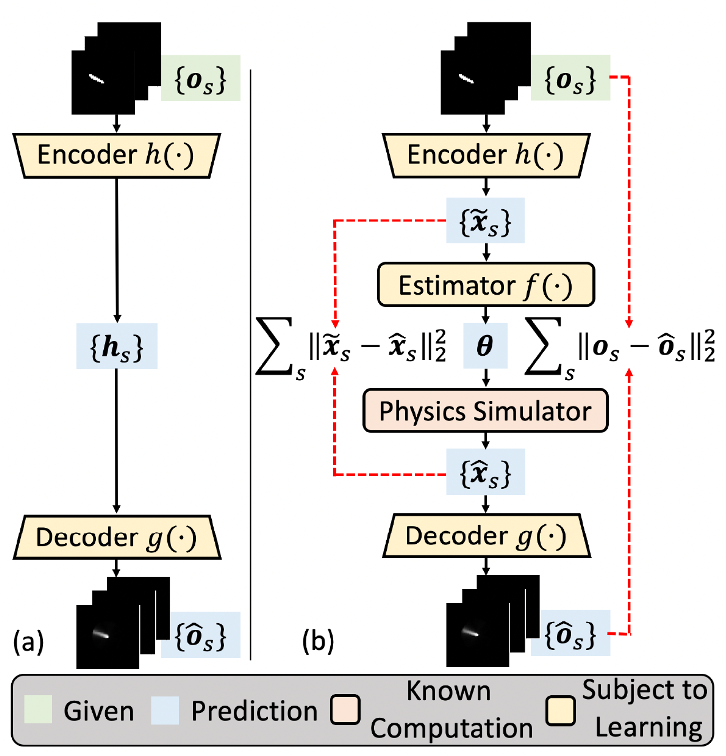
\includegraphics[width=0.45\textwidth]{architecture}
  \caption{ALPS Architecture}
  \label{fig:architecture}
\end{figure}
\\
\textbf{The encoder network.} The network estimates states $\tilde{x}_{s}$ from an observation sequence ${o_s}$. Depending on the type of observations --- pixel images or direct measurements --- a convolution or feedforward network is used to represent an observation ${o}$ as a vector embedding ${z'}$. To understand the dynamics within the data, the local and global context of the dynamics are extracted by aggregating the vector embedding ${z'}$ using a self-attention network~\cite{NIPS2017_3f5ee243}. Firstly, to incorporate positional information, a positional encoding is added to the embeddings which are then stacked over ${\tau}$ steps to form a matrix. Secondly, to calculate the attention softmax is taken over the ${\tau}$ steps. Thirdly, to allow the model to jointly attend to information from different representation subspaces at different positions the multi-head attention mechanism is applied (\ref{eq:multihead},\ref{eq:attention}).
\begin{equation}
  \label{eq:multihead}
  \text{Multihead} = \text{Concat}(\text{head}_1, \ldots, \text{head}_h) \cdot W^{O}
\end{equation}
\begin{equation}
  \label{eq:attention}
  \text{head}_i = \text{Attention}(Q, K, V) = \text{softmax}\left(\frac{{QK^T}}{\sqrt{d}}\right)V,
\end{equation}
where ${Q, K, V}$ represent the query, key, and value matrices of dimensionality ${d}$ respectively and $W^{O}$ are learnable matrices.\\
Finally, using Gaussian and Mises distributions as posterior for translational and rotational coordinates accordingly, a feedforward network produces the parameters of the distribution for each state in the sequence.
\\
\textbf{Analysis of self-attention mechanism.}
One possible direction for future work is to study the self-attention mechanism more precisely. To analyze NN attention we can visualize attention weights of a simple vehicle steering dynamics scenario~(\ref{eq:steering}) with the lateral path deviation ${x^{p}}$, turning rate ${x^{r}}$ and the input force to the steering wheel ${u}$. The network estimates ${x^{r}}$ from ${x^{p}}$ and vice versa. In the first case, the network attends to the neighboring observations at the current time (diagonal pattern) and performs derivative operation (local context). In the second case (Fig.~\ref{fig:integration}) the network attends to the observations from beginning to the current time (triangular pattern) and performs integration operation (global context).
\begin{equation}
  \label{eq:steering}
  \frac{dx}{dt} = 
  \begin{pmatrix}
  0 & 1 \\ 0 & 0 
  \end{pmatrix}
  x + 
  \begin{pmatrix}
  0.1 \\ 1 
  \end{pmatrix}
  u, \quad x = \begin{pmatrix} x^{p} \\ x^{r} \end{pmatrix}
\end{equation}
\begin{figure}
  \centering
  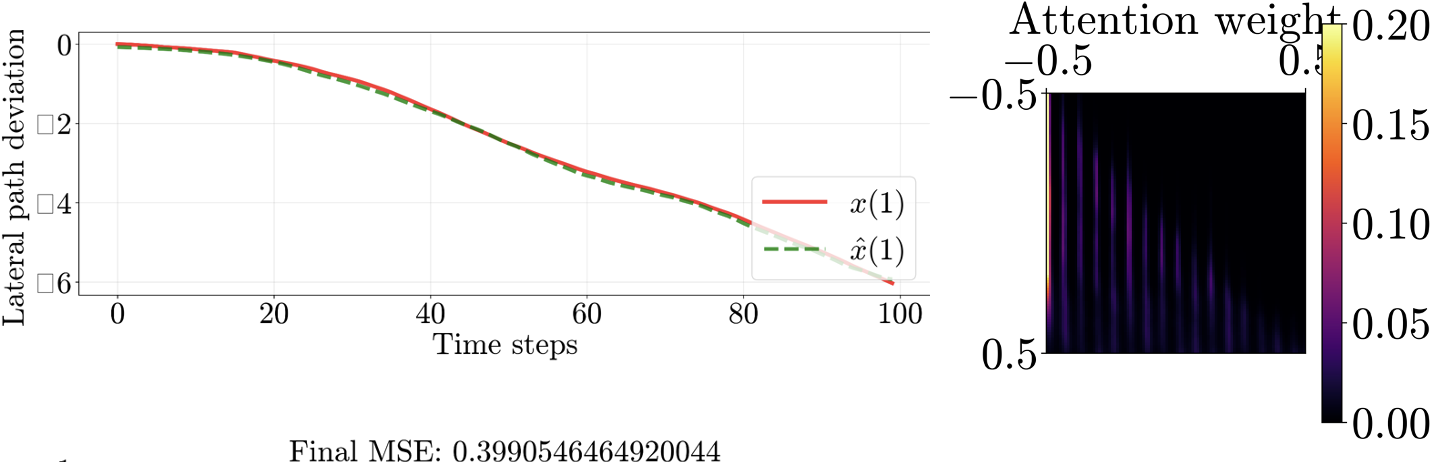
\includegraphics[width=0.35\textwidth]{integration}
  \caption{Estimation of literal path deviation from the turning rate}
  \label{fig:integration}
\end{figure}
\textbf{The parameter estimator network.} 
The network predicts physical parameters ${\theta}$  from the states $\tilde{x}_{s}$. It was shown that multilayer perceptrons (MLPs) are affected by spectral bias~\cite{rahamanspectral} i.e.~lower frequencies are learned first. Therefore, for systems that involve periodical or vibrational behavior, such as pendulum and oscillator, the input is passed through a Fourier transform on each component ${j}$ of state trajectory~(\ref{eq:fourier}) in order to capture high frequency content in the data~\cite{tancik2020ffn}. For systems, which do not have periodic behavior the transformation is not needed. For each Fourier feature mapping a residual network~\cite{7780459} is used to get a representation. The parameter estimator MLP network predicts physical parameters ${\theta}$ by taking a concatenation of the magnitudes of Fourier features ${|\tilde{X}_{\omega}(j)|}$ from states $\tilde{x}_{s}$.
\begin{equation}
  \label{eq:fourier}
  \tilde{X}_{\omega}(j) := \sum_{k=t-\tau+1}^{t} \tilde{x}_k(j) \left( \cos \left(\frac{2\pi}{\tau} \omega k \right) - i \cdot \sin \left(\frac{2\pi}{\tau} \omega k \right) \right)
\end{equation}
\textbf{The Neural Tangent Kernel theory.} The choice of using magnitudes of the Fourier features for periodic systems can be justified by estimating convergence rate of different Fourier feature mappings using neural tangent kernels~\cite{NEURIPS2018_5a4be1fa}. Consider a set of labelled training data $\{(v_i, y_i)\}_{i=1}^{m}$ with $v_i \in \mathbb{R}^n$, $y_i \in \mathbb{R}$, and $i \in [1 : m]$, where state trajectory is ${\mathbf{v} = [x_0, x_1, \ldots, x_{\tau-1}]^T}$ and ${\phi: \mathbb{R}^n \rightarrow \mathbb{R}^r}$ with kernel ${k(\mathbf{v}_i, \mathbf{v}_j) = (\mathbf{v}_i)^T (\mathbf{v}_j)}$ is a feature map. Set $\mathbf{y} = [y_1, \ldots, y_m]^T \in \mathbb{R}^m$, $K = [k(\mathbf{v}_i, \mathbf{v}_j)] \in \mathbb{R}^{m \times m}$ denote the kernel matrix for the training examples and $k(\mathbf{v}) = [k(\mathbf{v}_i, \mathbf{v})] \in \mathbb{R}^{m}$ denote the vector of kernel evaluations $k(\mathbf{v}_i, \mathbf{v})$, $i \in [1, m]$, for a test sample $\mathbf{v} \in \mathbb{R}^n$. The resulting kernel regression predictor is $\hat{y}(\mathbf{v}) = \mathbf{y}^T K^{-1} k(\mathbf{v})$.
According to the NTK theory when the number of neurons in each layer of fully-connected deep network with weights ${\mathbf{w}}$ initialized from a Gaussian distribution ${\mathcal{N}}$ tends to infinity, and the learning rate for stochastic gradient descent tends to zero, the neural network estimator ${\hat{y}(\mathbf{v};\mathbf{w})}$ converges to the kernel regression solution. 
\\
The studied feature maps include the Fourier feature mapping, their magnitudes and their phases~(\ref{eq:feature_maps}).
\begin{equation}
  \label{eq:feature_maps}
  \begin{aligned}
  \phi_{\text{DFT}}(\mathbf{v}) &= [X_0, \ldots, X!, \ldots, X_{\tau-1}]^T \in \mathbb{R}^\tau \\
  \phi_{\text{MAG}}(\mathbf{v}) &= [|X_0|, \ldots, |X_{\tau-1}|]^T \in \mathbb{R}^\tau \\
  \phi_{\text{PHA}}(\mathbf{v}) &= [\text{arg}(X_0), \ldots, \text{arg}(X_{\tau-1})]^T \in \mathbb{R}^\tau
  \end{aligned}
\end{equation}
Setting $C_k = [\cos \left(\frac{2\pi}{\tau} k_i 0\right) - \sin \left(\frac{2\pi}{\tau} k_j 0\right)] \in \mathbb{R}^{\tau \times \tau}$, the kernel functions of the mappings can be calculated the following way~(\ref{eq:fourier_kernels}).
\begin{equation} 
  \label{eq:fourier_kernels}
  \begin{aligned}
  & k_{\text{DFT}}(\mathbf{v}_1, \mathbf{v}_2) = \frac{1}{\tau} \sum_{k=0}^{\tau-1} \mathbf{v}_1^T C_k \mathbf{v}_2; \\
  & k_{\text{MAG}}(\mathbf{v}_1, \mathbf{v}_2) = \frac{1}{\tau} \sum_{k=0}^{\tau-1} \sqrt{\mathbf{v}_1^T C_k \mathbf{v}_1 \mathbf{v}_2^T C_k \mathbf{v}_2}; \\
  & k_{\text{PHA}}(\mathbf{v}_1, \mathbf{v}_2) = \phi_{\text{PHA}}(\mathbf{v}_1)^T \phi_{\text{PHA}}(\mathbf{v}_2).
  \end{aligned}
\end{equation}
In order to analyze the kernel spatial of different mapping we need to look at eigenvalues of corresponding kernel matrices of the composed NTK. Firstly, the kernel function is applied to every pair of samples from the trajectory ${\mathbf{v}}$. Secondly, the kernel regression is performed using the kernel matrix ${K}$ to predict the output ${\hat{y}(\mathbf{v})}$. Lastly, the NTK is computed ~(\ref{eq:kernel_ntk}).
\begin{equation}
  \label{eq:kernel_ntk}
  k_{\text{NTK}}(v_i, v_j) = \mathbb{E}_{w \sim \mathcal{N}} \left[ \nabla_{w} \hat{y}^{(t)}(v_i;w)^\top \nabla_{w} \hat{y}^{(t)}(v_j;w) \right]
\end{equation}
Large eigenvalues in the Neural Tangent Kernel (NTK) indicate sensitivity to small changes in the input space, facilitating the network's ability to capture fine-grained details and learn complex patterns in the data. Spatial plot shows that $k_{\text{MAG}}$ and $k_{\text{PHA}}$ have a slower decay in the high-frequency domain and therefore $k_{\text{MAG}}$ preserve most of the high-frequency components in the data (Fig.~\ref{fig:eigenvalues}).
\begin{figure}
  \centering
  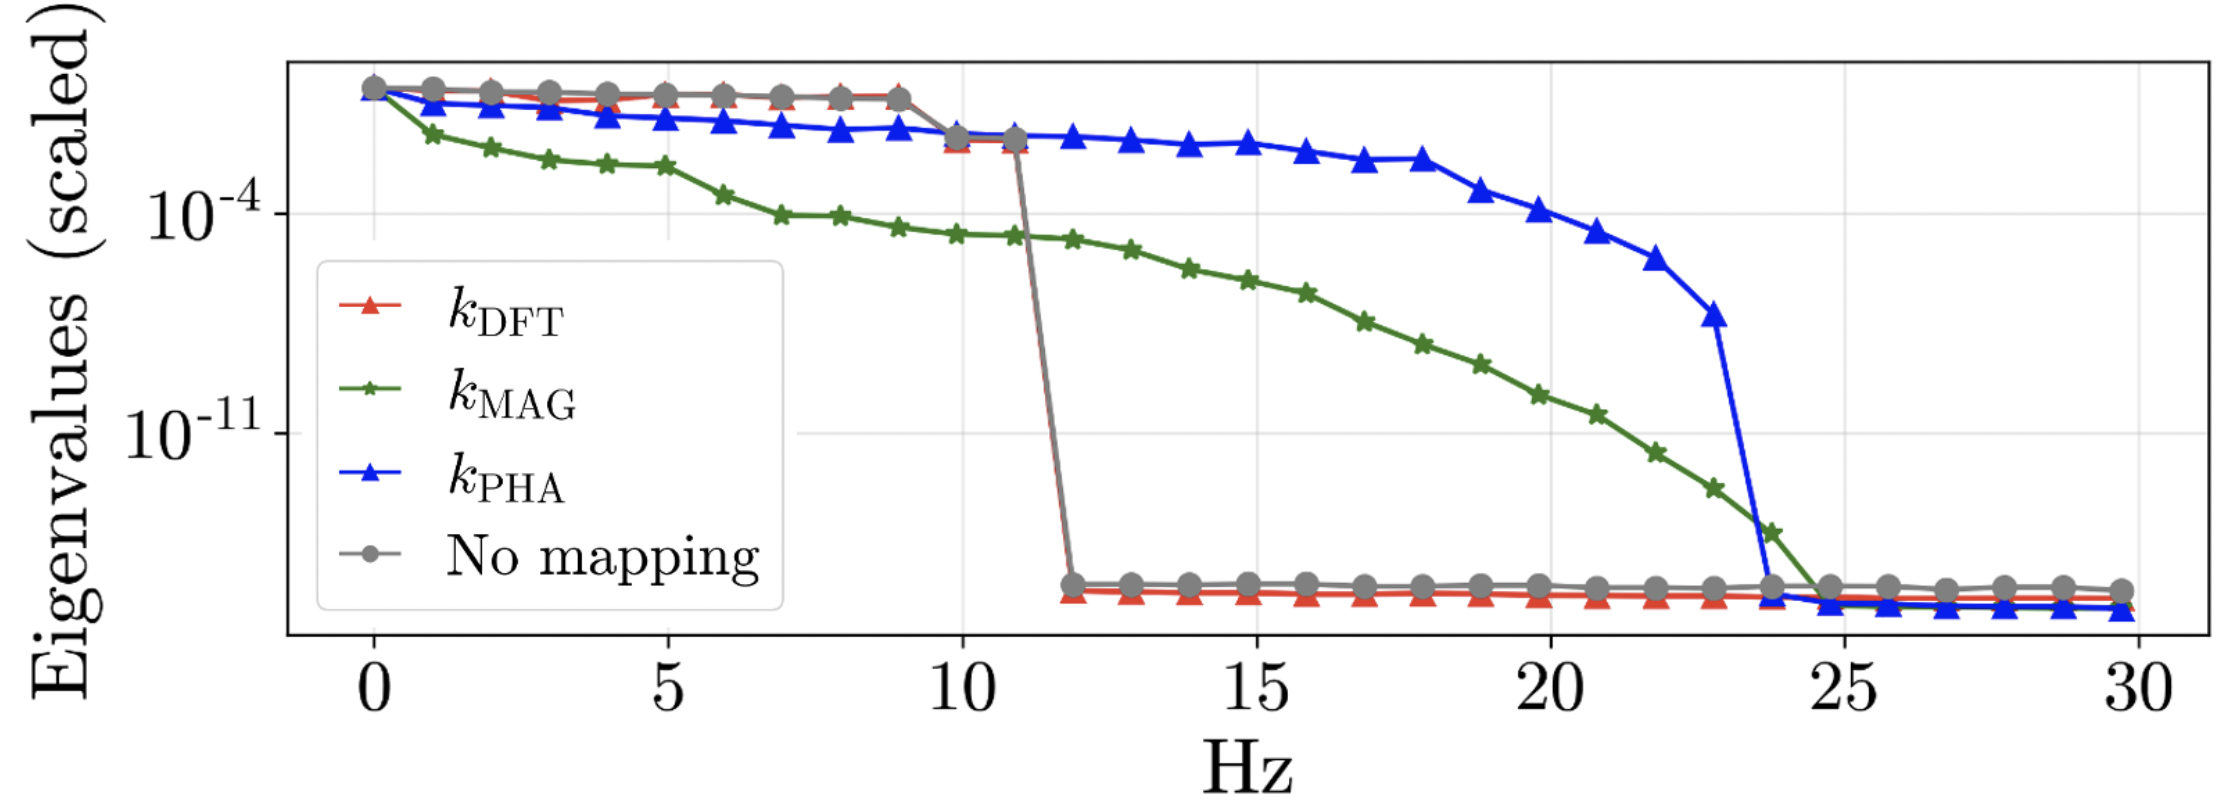
\includegraphics[width=0.45\textwidth]{eigenvalues}
  \caption{Kernel spatial of the kernel matrices}
  \label{fig:eigenvalues}
\end{figure}
\\
\textbf{The physics simulator.} The core of the physics simulator is a neural ordinary differential equation (ODE). Neural ODE~\cite{NEURIPS2018_69386f6b} is a type of neural network (NN) models, where instead of specifying a discrete sequence of hidden layers, the derivative of the hidden state is parameterized using a NN.\@ Given the initial state ${\tilde{x}_{s}}$ predicted by the encoder and physical parameters ${\theta}$ predicted by the estimator, the ODE solver rollouts state trajectories ${\hat{x}_s}$~(\ref{eq:ode_solver}).
\begin{align}
  \label{eq:ode_solver}
  & \{ \hat{x}_s \}_{s=t-\tau+1}^{t} : \hat{x}_{t-\tau+1}, \ldots, \hat{x}_{t-1}, \hat{x}_t \nonumber \\
  & = \text{ODESolver}( \tilde{x}_{t-\tau+1}, \dot{x} = A({\theta}) x + B({\theta}) u, \tau, \triangle ),
\end{align}
where ${\triangle}$ is a sampling start interval.
\\
\textbf{The decoder network.} Depending on the type of the input observations — images or sensor measurements — the decoder network is either a deconvolutional or a feedforward network, that generates a reconstructed observation ${\hat{o}_s}$ from each of the states ${\hat{x}_s}$, simulated by the ODE solver.
\\
\textbf{The loss function.} The loss function consists of three loses~(\ref{eq:loss_function}). Firstly, the variational autoencoder (VAE) loss is used to train the encoder ${h}$, the estimator ${f}$ and the decoder ${g}$. Secondly, the observation reconstruction loss used to minimize the error between input ${o_s}$ and reconstructed ${\hat{o}_s}$ observations, which improves the image reconstruction quality. Thirdly, the state reconstruction loss encourages states, defined by encoder ${\tilde{x}_{s}}$ to follow the ones, generated by physics simulator ${\hat{x}_s}$ and constrains the encoder from predicting arbitrary sequences.
\begin{equation}
  \label{eq:loss_function}
  \begin{aligned}
  L &= \sum_{s=t-\tau+1}^{t} D_{KL}(Q(\tilde{x}_s|o_s) || P(\tilde{x}_s)) \\
  &\quad + \sum_{s=t-\tau+1}^{t} \| o_s - \hat{o}_s \|_2^2 + \sum_{s=t-\tau+1}^{t} \| \tilde{x}_s - \hat{x}_s \|_2^2
  \end{aligned}
\end{equation}
where ${Q(\tilde{x}_s|o_s)}$ - posterior distribution, ${P(\tilde{x}_s)}$ - prior distribution, ${D_{KL}}$ - Kullback-Leibler divergence.
\section{Performance Evaluation}
To evaluate the ALPS performance and an effect of chosen self-attention and Fourier mapping mechanisms the following baselines methods were selected for comparison.
\begin{enumerate}
  \item Context-aware dynamics model (CaDM)~\cite{lee2020context}. This state-of-the-art method that decomposes the task of learning a global dynamics model into two stages: learning a context latent vector that captures the local dynamics and then predicting the next state conditioned on it.
  \item Autoencoder --- ALPS w/o estimator and physics simulator.
  \item ALPS w/o the Fourier feature mapping --- Fourier feature mapping is replaces with raw state trajectories ${\tilde{x}_{s}}$.
  \item ALPS w/o self-attention networks --- self-attention network in the encoder is replaced by a simple MLP.
\end{enumerate}
The models are compared based on three errors: state prediction error (SE), observation prediction error (OE) and parameter prediction error (PE) in solving the task of estimating physical parameters of three visual systems: pendulum, mass-spring-damper (MSD) and two-body. To generate a dataset, first, for each task initial state and physical parameters were sampled randomly, then 125 step rollout following the true system dynamics were rendered in a form of 64 by 64 by 3 pixel observation snapshots.
\begin{figure}
  \centering
  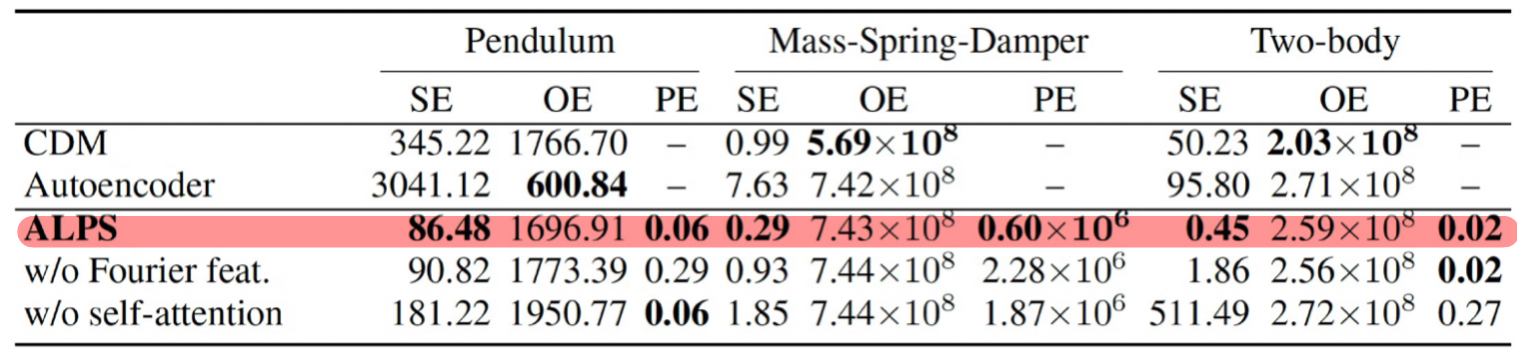
\includegraphics[width=0.45\textwidth]{ALPS_performance}
  \caption{Performance of tested networks in the visual tasks}
  \label{fig:performance}
\end{figure}
\\
The performance evaluation results shows (Fig.~\ref{fig:performance}) that ALPS reaches the best performance in predicting physical parameters utilizing both, self-attention and Fourier mapping. Moreover, Fourier feature mapping improves the results for pendulum, MSD, but two-body task, which proves using the mapping for systems that involve periodical or vibrational behavior. Regarding state predictions, ALPS achieves competitive results among the networks. In addition, it is visible that without self-attention networks, the SE increase drastically due to a large error in computing the velocity. Moreover, the high SE in the encoder network suggests that its latent representation is uninterpretable, which proves the idea of using physics to constrain the representation for estimating states in the encoder network. Lately, ALPS actives a comparable results in reconstructing observations. 
\section{ALPS Limitations}
\textbf{The first limitation} that make it challenging to apply ALPS to more complicated systems such as contact and fluid dynamics is the requirement for system to have a dynamic equation coupled with an assumption that the system is linear. The solution for this challenge might be found in combining known physics with neural models. One of the possible approaches is using interaction networks~\cite{battaglia2016interaction} as a neural model. The model can reason about how objects in complex systems interact, including dynamical predictions. For physical reasoning, the model takes a graph of objects and relations as input~\cite{scarselli2009graph}, reasons about their interactions, and applies the effects and physical dynamics to predict new states. Another approach is to use a framework for unsupervised meta-learning of hybrid latent dynamics~\cite{ye2024unsupervised} (Meta-HyLaD). The Meta-HyLaD consists of two parts: the first part is integrating established mathematical expressions representing prior physics with neural functions that capture unknown errors to form a latent dynamic function; the second part is employing a meta-learning framework aimed at discerning and separately characterizing both components within the hybrid dynamics.
\\
\textbf{The second limitation} is the requirement of neural ODE solver when simulating trajectories, which in addition results in high computational costs. The solution to the challenge might be found in using other technique to insert prior knowledge~\cite{botev2021which}. Using Hamiltonian Generative Networks (HGN)~\cite{toth2019hamiltonian} and Lagrangian Generative Networks (LGN)~\cite{lutter2019deep} as priors involves parameterizing kinetic and potential energies with neural networks. These networks, along with the encoder's latent state, enable simulating motion equations using numerical integrators like leap-frog for HGN and adaptive stepsize Runge-Kutta for LGN. Another approach is using Recurrent Generative Network (RGN)~\cite{chen2019symplectic} that uses the same MLP as the Neural ODE model but parametrizes the discrete state evolution in latent space. 
\section{Conclusions}
In this article we addressed the problem of predicting states and physical parameters of a system from observations with dynamic equations. By integrating an encoder, estimator, physics simulator, and decoder, ALPS enables the estimation of states and physical parameters from observations while adhering to the underlying laws of physics. The incorporation of self-attention mechanisms and Fourier mapping techniques, supported by the Neural Tangent Kernel theory, enhances the model's performance and interpretability. Despite its limitations, ALPS shows promising results and opens directions for extending the framework to handle more complex systems.

% Bibliography
\bibliographystyle{ACM-Reference-Format}
\bibliography{learning-physics}

\end{document}
